\chapter{Implementation of a combined PCI-interferometer on \diiid}


\section{Optical-diagnostic access on \diiid}
\label{sec:Implementation:d3d_ports}
\diiid \space provides optical access to its plasmas
through a number of ports, as indicated in
Fig.~\ref{fig:Implementation:d3d_port_locations}.
The ports are labeled according to their
toroidal positions and their sightlines, and
an experimentalist should have at least
a rough familiarity with these conventions.
The toroidal location of a port
is given in degrees clockwise from ``machine north''
when viewing the machine from above
(note that machine north does \emph{not} correspond
to geographic or magnetic north).
The angular separation of adjacent toroidal ports is $15^{\circ}$.
Port sightlines can be vertical or radial.
Ports with vertical (V) sightlines
are labeled sequentially in terms of increasing major radius,
with $V1$ having the smallest major radius and
$V3$ having the largest major radius.
Radial ports (R) have sightlines
that are roughly aligned with the plasma's minor radius, and
they are labeled according to their positions
relative to the plasma midplane:
R0 sits at the plasma midplane,
R+1 and R+2 are the first and second ports
\emph{above} the plasma midplane, respectively, and
R-1 and R-2 are the first and second ports
\emph{below} the plasma midplane, respectively.

\begin{figure}
  \centering
  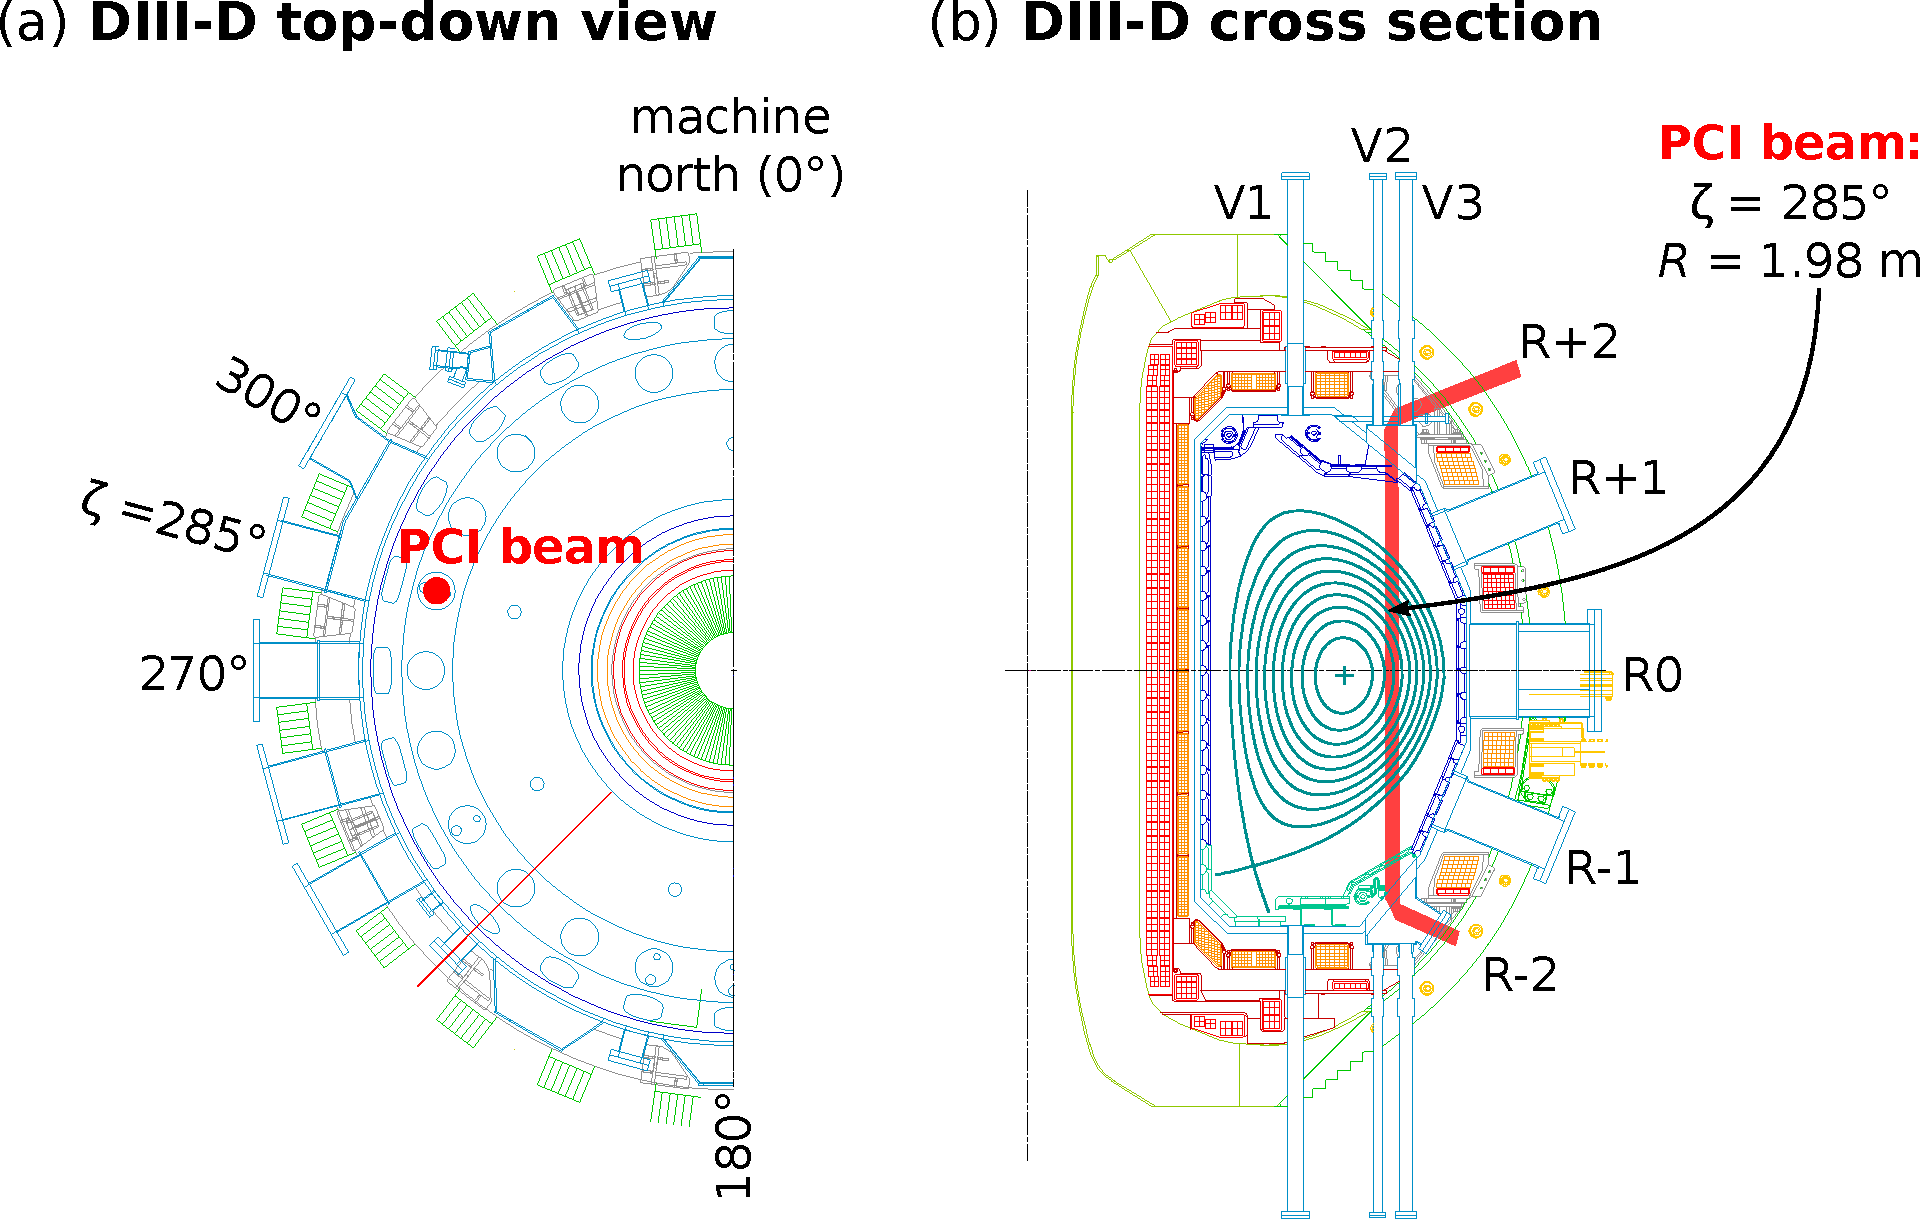
\includegraphics[width = \textwidth]{%
    Chapters/Implementation/figs/d3d_port_locations.pdf}
  \caption[\diiid \space port-labeling conventions and location of PCI]{%
    (a) View of \diiid \space from above,
    indicating the toroidal-labeling convention.
    (b) View of \diiid \space cross section,
    indicating the labeling convention
    for vertical (V) and radial (R) sightlines.
    The PCI beam enters the vessel through the $285^{\circ}$ R+2 port,
    propagates vertically downwards through the plasma
    at a major radius of $R = \SI{1.98}{\meter}$, and
    exits the vessel through the $285^{\circ}$ R-2 port.}
\label{fig:Implementation:d3d_port_locations}
\end{figure}


\section{\diiid's pre-existing PCI system}
The \diiid \space PCI system is
thoroughly described elsewhere~\cite{dorris_rsi09, dorris_phd}, but
the system components of relevance to this work
are briefly summarized below for completeness.


\subsection{System geometry}
The system is currently configured
in the ``Phase II'' geometry~\cite{dorris_rsi09},
with the probe beam propagating vertically downwards
from the $285^{\circ}$ R+2 port to the $285^{\circ}$ R-2 port.
The beam center sits at $R = $ \SI{1.98}{\meter}.
Both the toroidal and radial positions
of the PCI beam are shown in
Fig.~\ref{fig:Implementation:d3d_port_locations}.

The PCI system's vertical beam path constrains
which types of fluctuations it can and cannot detect.
Namely, the PCI-measured power fluctuations
(\ref{eq:InterferometricMethods:PCI_ratio_fluctuating_to_equilibrium_power})
correspond to \emph{line-integrated} electron-density fluctuations, which
are the physical origin of the phase fluctuations $\tilde{\phi}$ in
(\ref{eq:InterferometricMethods:phase_fluctuation}).
Because it is a line-integrated measurement,
only fluctuations propagating perpendicular to the beam path can be detected,
as fluctuations propagating parallel to the beam path
are effectively averaged out of the signal
\graffito{\textcolor{red}{what about $\delta \omega$?}}
(and, at a more fundamental level, fluctuations propagating
parallel to the beam path do \emph{not} spatially scatter the probe beam).
\graffito{\textcolor{red}{citation? Wesson?}}
Now, electrostatic turbulence (e.g.\ ITG, ETG) tends to be field-aligned
such that $k_{\perp} \gg k_{||}$, where
the $\perp$ and $||$ subscripts are used here to indicate
orientations that are perpendicular to and parallel to
the local magnetic field, respectively.
To lowest order, then, electrostatic fluctuations propagate
perpendicular to a tokamak's toroidal field.
PCI's vertical beam path and
the field-aligned constraint of electrostatic turbulence
imply that PCI is predominantly sensitive to fluctuations
with finite major-radial wavenumber $k_R$.
Thus, PCI's 32-element, 1-dimensional detector array
is oriented in the image plane such that
each detector element corresponds to a unique major radius in the plasma.

In some situations, spatially filtering ``masks''
\cite{dorris_rsi09, dorris_phd, lin_rsi06} or
2-dimensional detector arrays
\cite{sanin_rsi04, tanaka_rsi16}
can be used to localize measurements
by exploiting the spatial variation
in the magnetic field's orientation along the beam path.
These localization techniques typically work best
for high-$k$ measurements.
Note that $k_R$ is related to the
often-theoretically-relevant poloidal wavenumber $k_{\theta}$ via
\begin{equation}
  k_R = k_{\theta} \csc[\alpha(R, z)],
  \label{eq:Implementation:kR_to_ktheta}
\end{equation}
where $\alpha(R, z)$ is the angle
between the beam path and the local flux surface,
as shown schematically in
Fig.~\ref{fig:Implementation:relating_kR_to_ktheta}.
Of course, the fluctuation measurements must be localized,
either via direct measurement
(with 2-dimensional detector arrays or ``masks'')
or via inference from other plasma properties,
before (\ref{eq:Implementation:kR_to_ktheta})
can be inverted to yield $k_{\theta}$
from measured values of $k_R$.

\begin{figure}
  \centering
  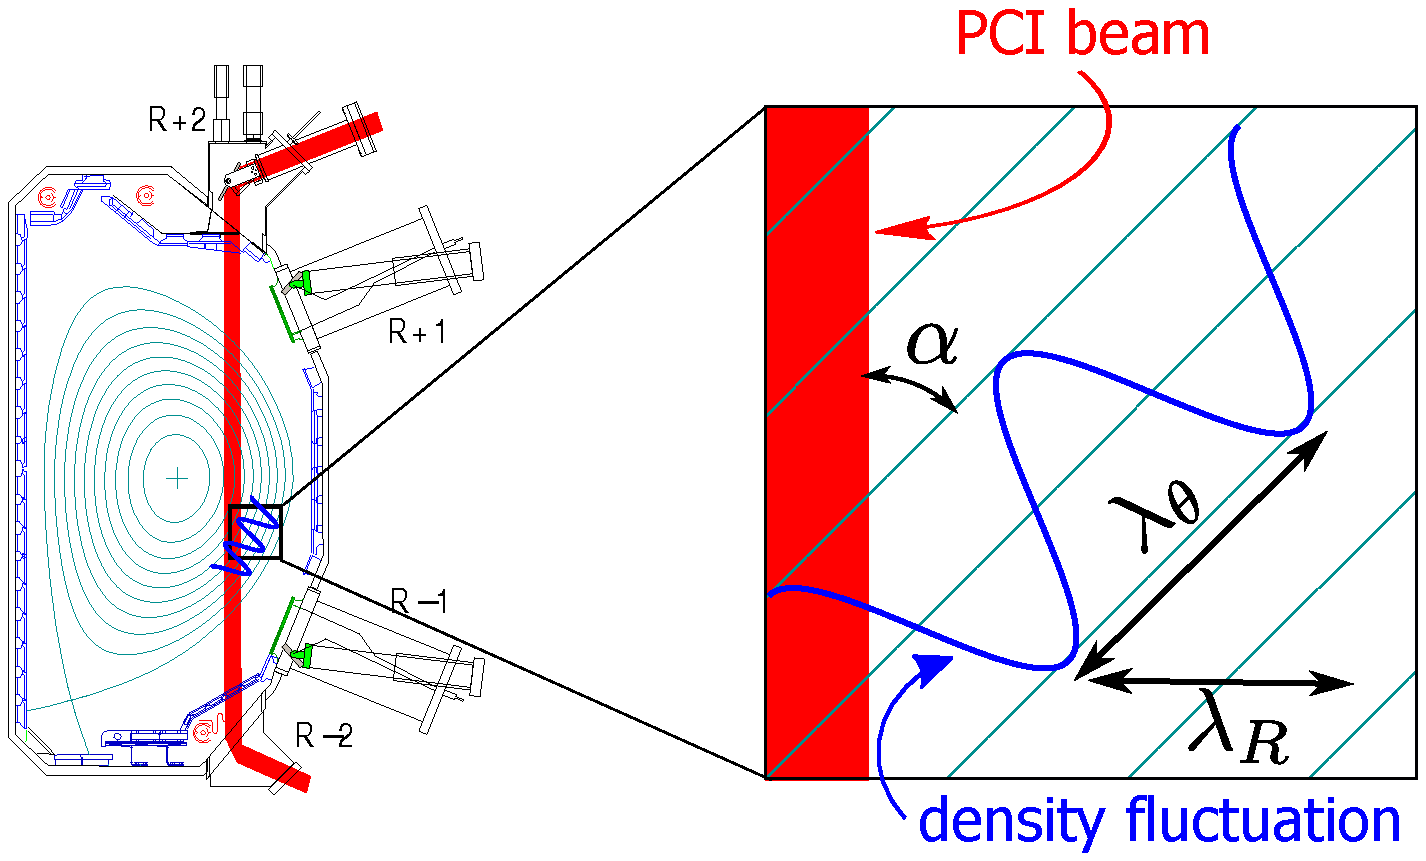
\includegraphics[width = 0.9 \textwidth]{%
    Chapters/Implementation/figs/kR_to_ktheta.pdf}
  \caption[Relating $k_R$ to $k_{\theta}$]{%
    The major-radial wavenumber $k_R = 2 \pi / \lambda_R$ and
    the poloidal wavenumber $k_{\theta} = 2 \pi / \lambda_{\theta}$
    are related via $\alpha(R, z)$, which
    is the angle between PCI's vertical probe beam and
    the local flux surface.}
\label{fig:Implementation:relating_kR_to_ktheta}
\end{figure}


\subsection{Spatial bandwidth}
Several critical wavenumbers were defined in
Section~\ref{sec:InterferometricMethods:pci} that
characterize the spatial bandwidth of a PCI system.
The goal of this section is to evaluate each of these
wavenumbers with the relevant parameters from
the \diiid \space PCI system.

PCI's low-$k$ cutoff, $k_g$, is physically constrained by
the free-space diffraction of the in-vessel probe beam.
This constraint was derived both
by examining the far-field overlap of the scattered and unscattered beams as in
(\ref{eq:InterferometricMethods:kmin_for_far_field_beam_separation}) and
by matching the spot size of the focused, unscattered beam
on the phase plate with the width of the phase plate's groove as in
(\ref{eq:InterferometricMethods:pci_kmin_physics}).
Both approaches yield the identical constraint that
$k_g^{\text{min}} = 2 / w_0$, where
$w_0$ is the 1/e $E$ radius of the in-vessel probe beam.
Capping aperture diffraction at acceptably small levels, however,
yields constraint
(\ref{eq:InterferometricMethods:aperture_radius_for_minimal_diffraction})
on $w_0$.
Now, after beam expansion and collimation,
the smallest aperture prior to beam-plasma interaction
is the $285^{\circ}$ R+2 port window,
which has a diameter of $4"$.
Thus, the beam expansion optics are configured to produce
to produce the widest possible beam
\begin{equation}
  w_0 = 4/3" \approx \SI{3.4}{\centi\meter}
\end{equation}
and the smallest physical constraint on the PCI low-$k$ cutoff
\begin{equation}
  k_g^{\text{min}} \approx \SI{0.6}{\per\centi\meter}
  \label{eq:Implementation:kg_min}
\end{equation}
while introducing negligible aperture diffraction.

PCI's \emph{realized} low-$k$ cutoff, however,
is typically $\sim 2-3 \times$ larger than
the diffraction-limited $k_g^{\text{min}}$.
This occurs if the width of the phase-plate groove
is oversized relative to the focused, unscattered beam spot, and
the realized low-$k$ cutoff is given by
(\ref{eq:InterferometricMethods:pci_kmin_engineering}).
Despite sacrificing some of the system's low-$k$ range,
operating with an oversized phase-groove width can be advantageous
on large, vibration-prone fusion experiments.
To see this, recall that the phase groove typically reflects
only a fraction $\eta < 1$ of the incident unscattered beam power
(the forward-facing surface of the \diiid \space phase-plate groove
is uncoated ZnSe, which has $\eta = 0.17$ at $\SI{10.6}{\micro\meter}$);
if vibration-induced misalignments
push the unscattered beam out of the phase groove,
there will be large power modulations on the PCI detector
that are \emph{not} attributable to plasma fluctuations and
that push the detector beyond its saturation limits.
While \diiid's PCI system has an elaborate feedback control system
that dynamically centers the unscattered beam on the phase-plate groove
\cite[Sec.~3.5]{coda_phd},
operating with an oversized phase-groove width
increases the size of the ``targeted'' operating space,
effectively giving the feedback system some leeway.
As such, the groove width of the \diiid \space phase plate is
\begin{equation}
  d = \SI{1}{\milli\meter},
\end{equation}
and the scattered beams are focused onto the phase plate by
an off-axis parabolic mirror of focal length
\begin{equation}
  f = 80.7"
\end{equation}
such that the realized low-$k$ cutoff
(\ref{eq:InterferometricMethods:pci_kmin_engineering})
becomes
\begin{equation}
  k_g \approx \SI{1.5}{\per\centi\meter},
\end{equation}
approximately $2.5 \times$ larger than
the diffraction-limited minimum in (\ref{eq:Implementation:kg_min}).

PCI's high-$k$ limits are dictated by
finite-sized collection optics and system magnification.
The \diiid \space phase plate has a diameter
\begin{equation}
  D = 2"
\end{equation}
such that the phase plate's high-$k$ cutoff
(\ref{eq:InterferometricMethods:pci_kmax_engineering})
is
\begin{equation}
  k_D \approx \SI{75}{\per\centi\meter}.
\end{equation}
Although the $5"$ diameter $285^{\circ}$ R-2 exit window and
the subsequent $12"$ diameter steering mirrors
are large enough to accommodate beams scattered
from fluctuations with wavenumbers $|k| \sim k_D$,
apertures in the imaging optics
only allow beams scattered from fluctuations with
\begin{equation}
  |k| \lesssim \SI{20}{\per\centi\meter}
\end{equation}
to reach the PCI detector.
Upon reaching the detector,
the measured PCI signal is subject to finite sampling-volume effects,
which result from spatial averaging over the face of a detector element.
The PCI's 32-element, 1-dimensional detector array have elements
of height $\SI{1}{\milli\meter}$, width
\begin{equation}
  s_x^{\text{pci}} = \SI{0.5}{\milli\meter},
\end{equation}
and center-to-center element spacing of $\SI{0.55}{\milli\meter}$.
Coupled with the system's magnification
\graffito{\textcolor{red}{Correct? Sign?}}
\begin{equation}
  |M^{\text{pci}}| \approx 0.5,
\end{equation}
the finite sampling-volume cutoff
(\ref{eq:InterferometricMethods:finite_sampling_volume_cutoff})
of the PCI is
\begin{equation}
  k_{\text{fsv}}^{\text{pci}} \approx \SI{63}{\per\centi\meter}.
\end{equation}


\subsection{Temporal bandwidth}
PCI's detector (Infrared Associates MCT-16-32) and
its associated preamplifiers (also through Infrared Associates)
are the dominant constraint on the system's temporal bandwidth.
The HgCdTe detector array
operates in the photoconductive regime and
is cooled by liquid nitrogen;
the liquid-nitrogen cooling reduces noise and boosts the response such that
the detector-preamplifier combination has
a specific detectivity
$D^* \approx \SI{2e10}{\centi\meter \sqrt\hertz \per\watt}$ and
a $\SI{500}{\volt\per\watt}$ responsivity
to incident $\SI{10.6}{\micro\meter}$ light
(note that the detector also has a saturation intensity
$I_{\text{sat}} \sim \SI{1}{\milli\watt \per\milli\meter\squared}$).
The benefits of cooling, however, come at the expense of reduced bandwidth:
the detector-preamplifier combination has
a high-frequency, 2-pole cutoff
at $\sim \SI{800}{\kilo\hertz}$~\cite{rost_pci_detector_response}.
As the DC PCI signal is of little interest,
the detector-preamplifier combination also has
a low-frequency, 1-pole cutoff
at $\sim \SI{2}{\kilo\hertz}$~\cite{rost_pci_detector_response}.

The components downstream of the detector and preamplifiers
have a small impact on the system bandwidth, but
they are briefly summarized below for completeness.
The Variable Gain and Filter (VGAF) circuits~\cite[Sec.~3.3.3]{dorris_phd}
are located immediately downstream of the preamplifiers and
have a low-frequency, 1-pole cutoff that can be easily switched between
$\SI{10}{\kilo\hertz}$ and $\SI{100}{\kilo\hertz}$;
the VGAFs are typically operated in the $\SI{10}{\kilo\hertz}$ configuration.
Following the VGAFs,
fiber optic links (Analog Modules 732 T/R-2.5-33k)
with an analog bandwidth of DC to $\SI{10}{\mega\hertz}$
transmit the signal from the \diiid \space pit to the annex.
Upon reaching the annex,
the signals are digitized with two of D-tAcq's ACQ216CPCI boards,
typically at a sampling rate of $f_s = 4 \, \text{MSPS}$.


\section{Component replacement}
Over the course of this work,
several components crucial to the operation of the PCI
(and the soon-to-be-described interferometer)
failed.
The failures and replacements are briefly described below.


\subsection{Quadrature detector for beam-position feedback}
A quadrature detector measures the position
of the unscattered beam on the phase plate,
providing the input to the feedback control system
that dynamically centers the unscattered beam
on the phase-plate groove~\cite[Sec.~3.5]{coda_phd}.
As the quadrature detector
cannot physically be co-located with the phase plate,
a beam splitter samples the unscattered beam
immediately upstream of the phase plate, and
a single lens \emph{images} onto the quadrature detector
the point in the sampled beam that corresponds to the phase-plate location.
Thus, beam movement on the phase plate is mirrored
by movement of the sampled beam on the quadrature detector.
System response is maximized
with imaging magnification $|M| \approx 1$
(relative to the beam size at the phase plate) and
incident optical intensities $I_{\text{opt}}$
well beyond the linear saturation intensity
(i.e. $I_{\text{sat}} \ll I_{\text{opt}} < I_{\text{dam}}$)
~\cite{marinoni_FB_detector_report}~\cite[Sec.~3.5(b)]{coda_phd}.

The old quadrature detector consisted of four
photoconductive, liquid-nitrogen cooled, HgCdTe elements.
Quadrature detectors for use at $\SI{10.6}{\micro\meter}$
had only just become commercially available
when this unit was procured from Belov Technology in the mid-1990s
~\cite[Sec.~3.5(b)]{coda_phd}.
Cooling HgCdTe can
extend the long-wavelength cutoff beyond $\SI{10.6}{\micro\meter}$,
reduces noise, and
increases responsivity~\cite{vigo_catalog}.
In particular, HgCdTe's responsivity increases by $\sim 10^3$
when cooled to liquid-nitrogen temperatures such that
that the incident optical signal
exceeds the $1 / f$ noise
characteristic of photoconductive detectors~\cite{vigo_catalog}.
As the bandwidth requirements for the PCI feedback system
extend from DC to $\lesssim \SI{10}{\kilo\hertz}$,
$1 / f$ noise cannot be easily combated by
e.g.\ mechanically chopping the beam.
After $\sim 20$ years of operation,
the old quadrature detector failed in December 2014,
presumably having reached its expected lifetime.
Fortunately, in the context of position sensing,
HgCdTe technology has significantly improved since the mid-1990s.

The new quadrature detector
(four VIGO PVM-10.6 elements mounted on a VIGO QIP preamplifier)
is in many ways superior to the old quadrature detector.
This superiority stems from VIGO's use of
``multiple heterojunction'' HgCdTe detector elements~\cite{vigo_catalog},
which endow the detector with several advantageous properties.
First, the detector is photovoltaic.
Thus, the detector is \emph{not} plagued by the $1 / f$ noise
characteristic of photoconductive detectors.
Second, the detector's long-wavelength cutoff
sits beyond $\SI{10.6}{\micro\meter}$ at room temperature.
Taken together, the above two properties imply that
the new quadrature detector can be operated at room temperature,
i.e.\ it does \emph{not} need to be cooled by liquid nitrogen.
Lacking a dewar, the new quadrature detector
is much smaller than the old quadrature detector;
the new detector can also be mounted with an arbitrary orientation,
whereas the dewar of the old detector required an upright orientation.
This new-found flexibility substantially opened
the optical design space for the feedback arm and
the plasma arm of the soon-to-be-described interferometer.
Additionally, the dewar of the old quadrature detector
only had a $\sim \SI{6}{\hour}$ hold time,
which is not sufficient for a full day of \diiid \space operations;
thus, the use of a room-temperature quadrature detector has
eliminated the mid-day ``pit runs'' to refill the quadrature detector's dewar,
allowing easier operation of the system.
Although room-temperature operation reduces
the detector's specific detectivity to
$D^* \sim \SI{e7}{\centi\meter \sqrt\hertz \per\watt}$
(roughly three orders of magnitude \emph{lower} than
that of the old quadrature detector),
the optical signal corresponds to the strong, unscattered probe beam
(as opposed to e.g.\ weak beams
scattered from small-amplitude plasma fluctuations), so
the increase in noise negligibly influences operation of the feedback system.

\begin{itemize}
  \item \textcolor{red}{Picture}
  \item \textcolor{red}{Table of properties (?)}
\end{itemize}


\subsection{Laser}
\subsection{In-vessel mirrors}


\section{Interferometer design}
\begin{itemize}
  \item Power sharing between the interferometer arms and PCI
  \item TE-cooled detector
  \item Imaging and $k$-response
  \item Demodulation scheme
\end{itemize}

\section{Interferometer optimization}
\begin{itemize}
  \item LO stability
  \item External clock
\end{itemize}

\section{Sound-wave calibration of combined PCI-interferometer}
\begin{itemize}
  \item Importance of speaker placement
  \item System sensitivity
\end{itemize}


\bibliographystyle{plainurl}
\bibliography{references}
